\documentclass[11pt,compress,t,notes=noshow, xcolor=table]{beamer}
\usepackage[]{graphicx}\usepackage[]{color}
% maxwidth is the original width if it is less than linewidth
% otherwise use linewidth (to make sure the graphics do not exceed the margin)
\makeatletter
\def\maxwidth{ %
  \ifdim\Gin@nat@width>\linewidth
    \linewidth
  \else
    \Gin@nat@width
  \fi
}
\makeatother

\definecolor{fgcolor}{rgb}{0.345, 0.345, 0.345}
\newcommand{\hlnum}[1]{\textcolor[rgb]{0.686,0.059,0.569}{#1}}%
\newcommand{\hlstr}[1]{\textcolor[rgb]{0.192,0.494,0.8}{#1}}%
\newcommand{\hlcom}[1]{\textcolor[rgb]{0.678,0.584,0.686}{\textit{#1}}}%
\newcommand{\hlopt}[1]{\textcolor[rgb]{0,0,0}{#1}}%
\newcommand{\hlstd}[1]{\textcolor[rgb]{0.345,0.345,0.345}{#1}}%
\newcommand{\hlkwa}[1]{\textcolor[rgb]{0.161,0.373,0.58}{\textbf{#1}}}%
\newcommand{\hlkwb}[1]{\textcolor[rgb]{0.69,0.353,0.396}{#1}}%
\newcommand{\hlkwc}[1]{\textcolor[rgb]{0.333,0.667,0.333}{#1}}%
\newcommand{\hlkwd}[1]{\textcolor[rgb]{0.737,0.353,0.396}{\textbf{#1}}}%
\let\hlipl\hlkwb

\usepackage{framed}
\makeatletter
\newenvironment{kframe}{%
 \def\at@end@of@kframe{}%
 \ifinner\ifhmode%
  \def\at@end@of@kframe{\end{minipage}}%
  \begin{minipage}{\columnwidth}%
 \fi\fi%
 \def\FrameCommand##1{\hskip\@totalleftmargin \hskip-\fboxsep
 \colorbox{shadecolor}{##1}\hskip-\fboxsep
     % There is no \\@totalrightmargin, so:
     \hskip-\linewidth \hskip-\@totalleftmargin \hskip\columnwidth}%
 \MakeFramed {\advance\hsize-\width
   \@totalleftmargin\z@ \linewidth\hsize
   \@setminipage}}%
 {\par\unskip\endMakeFramed%
 \at@end@of@kframe}
\makeatother

\definecolor{shadecolor}{rgb}{.97, .97, .97}
\definecolor{messagecolor}{rgb}{0, 0, 0}
\definecolor{warningcolor}{rgb}{1, 0, 1}
\definecolor{errorcolor}{rgb}{1, 0, 0}
\newenvironment{knitrout}{}{} % an empty environment to be redefined in TeX

\usepackage{alltt}
\newcommand{\SweaveOpts}[1]{}  % do not interfere with LaTeX
\newcommand{\SweaveInput}[1]{} % because they are not real TeX commands
\newcommand{\Sexpr}[1]{}       % will only be parsed by R



\usepackage[english]{babel}
\usepackage[utf8]{inputenc}

\usepackage{dsfont}
\usepackage{verbatim}
\usepackage{amsmath}
\usepackage{amsfonts}
\usepackage{bm}
\usepackage{csquotes}
\usepackage{multirow}
\usepackage{longtable}
\usepackage{booktabs}
\usepackage{enumerate}
\usepackage[absolute,overlay]{textpos}
\usepackage{psfrag}
\usepackage{algorithm}
\usepackage{algpseudocode}
\usepackage{eqnarray}
\usepackage{arydshln}
\usepackage{tabularx}
\usepackage{placeins}
\usepackage{tikz}
\usepackage{setspace}
\usepackage{colortbl}
\usepackage{mathtools}
\usepackage{wrapfig}
\usepackage{bm}
\usetikzlibrary{shapes,arrows,automata,positioning,calc,chains,trees, shadows}
\tikzset{
  %Define standard arrow tip
  >=stealth',
  %Define style for boxes
  punkt/.style={
    rectangle,
    rounded corners,
    draw=black, very thick,
    text width=6.5em,
    minimum height=2em,
    text centered},
  % Define arrow style
  pil/.style={
    ->,
    thick,
    shorten <=2pt,
    shorten >=2pt,}
}
\usepackage{subfig}


% Defines macros and environments
% basic latex stuff
\newcommand{\pkg}[1]{{\fontseries{b}\selectfont #1}} % fontstyle for R packages

% Often used in exercise Rnw files, still relevant?
\newcommand{\lz}{\vspace{0.5cm}} % vertical space
\newcommand{\dlz}{\vspace{1cm}}  % double vertical space

% Unused and about to be deleted
\newcommand{\oneliner}[1] % Oneliner for important statements
{\begin{block}{}\begin{center}\begin{Large}#1\end{Large}\end{center}\end{block}}


%--------------------%
%  New environments  %
%--------------------%

 % Frame with breaks and verbatim // this is used very often
\newenvironment{vbframe}
{
\begin{frame}[containsverbatim,allowframebreaks]
}
{
\end{frame}
}

% Frame with verbatim without breaks (to avoid numbering one slided frames)
% This is not used anywhere but I can see it being useful
\newenvironment{vframe}
{
\begin{frame}[containsverbatim]
}
{
\end{frame}
}

% Itemize block
\newenvironment{blocki}[1]
{
\begin{block}{#1}\begin{itemize}
}
{
\end{itemize}\end{block}
}

%--------------%
%  Citebutton  %
%--------------%
% Example usage (from slides-cart-discussion.tex)
% \citebutton{Breiman, 1984}{https://www.taylorfrancis.com/books/mono/10.1201/9781315139470/classification-regression-trees-leo-breiman}
\newcommand{\citebutton}[2]{%
\NoCaseChange{\resizebox{!}{9pt}{\protect\beamergotobutton{\href{#2}{#1}}}}%
}

% textcolor that works in mathmode
% https://tex.stackexchange.com/a/261480
% Used e.g. in forests/slides-forests-bagging.tex
% [...] \textcolor{blue}{\tfrac{1}{M}\sum^M_{m} [...]
\makeatletter
\renewcommand*{\@textcolor}[3]{%
  \protect\leavevmode
  \begingroup
    \color#1{#2}#3%
  \endgroup
}
\makeatother


%\usetheme{lmu-lecture}
\usepackage{../../style/lmu-lecture}

\let\code=\texttt
\let\proglang=\textsf

\setkeys{Gin}{width=0.9\textwidth}

\title{Introduction to Machine Learning}
% \author{Bernd Bischl, Christoph Molnar, Daniel Schalk, Fabian Scheipl}
\institute{\href{https://compstat-lmu.github.io/lecture_i2ml/}{compstat-lmu.github.io/lecture\_i2ml}}
\date{}

\setbeamertemplate{frametitle}{\expandafter\uppercase\expandafter\insertframetitle}



\begin{document}


% Load all R packages and set up knitr

% This file loads R packages, configures knitr options and sets preamble.Rnw as parent file
% IF YOU MODIFY THIS, PLZ ALSO MODIFY setup.Rmd ACCORDINGLY...







%! includes: tuning-nestedintro

\lecturechapter{Tuning: Training - Validation - Test}
\lecture{Introduction to Machine Learning}

\begin{frame}{Tuning Problem}

\vskip 3em
Remember:\\
\vskip 3em
We need to 

\begin{itemize}
\item \textbf{select an optimal learner} 
\item without compromising the \textbf{accuracy of the performance estimate} for that learner
\end{itemize}

-- for that we need an \textbf{untouched test set}!

\end{frame}

\begin{vbframe}{Train - Validation - Test}
Simplest method to achieve this: a 3-way split
\begin{itemize}
\item During tuning, a learner is trained on the \textbf{training set},
  evaluated on the  \textbf{validation set}
\item After the best model configuration $\lambda^\star$ is selected, we re-train on the joint (training+validation) set and evaluate the model's performance on the \textbf{test set}.
\end{itemize}
\begin{center}
% FIGURE SOURCE: https://docs.google.com/presentation/d/1kBxfxdUzyUP2-_Y5kWWJ1TnWsm-C4AjHQeTaYPeFo24/edit?usp=sharing
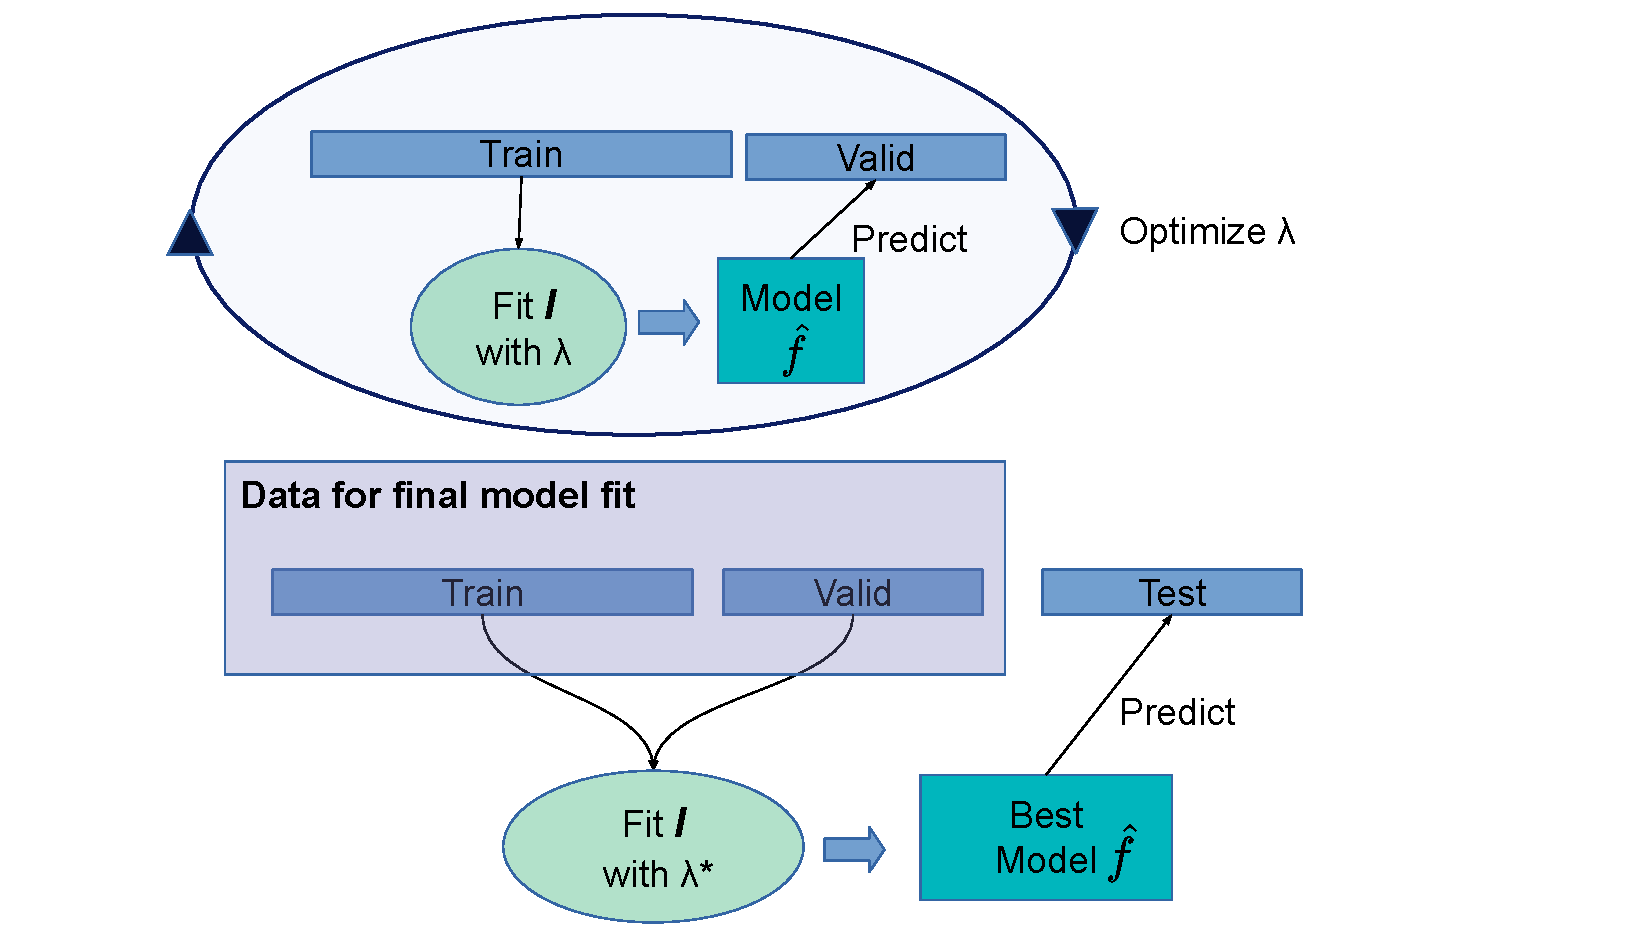
\includegraphics[width=0.7\textwidth]{figure_man/train_valid_test.pdf}
\end{center}
\end{vbframe}


\begin{vbframe}{Tuning as part of model building}
\begin{itemize}
\item Effectively, the tuning step is now simply part of a more complex training procedure.
\item We could see this as removing the hyperparameters from the inputs of the algorithm and making it \enquote{self-tuning}.
\end{itemize}
\begin{center}
% FIGURE SOURCE: https://docs.google.com/presentation/d/1JUtguuVBgidcqD0IdFFIiKH9zqYzM6YRjCqC53V90dA/edit?usp=sharing
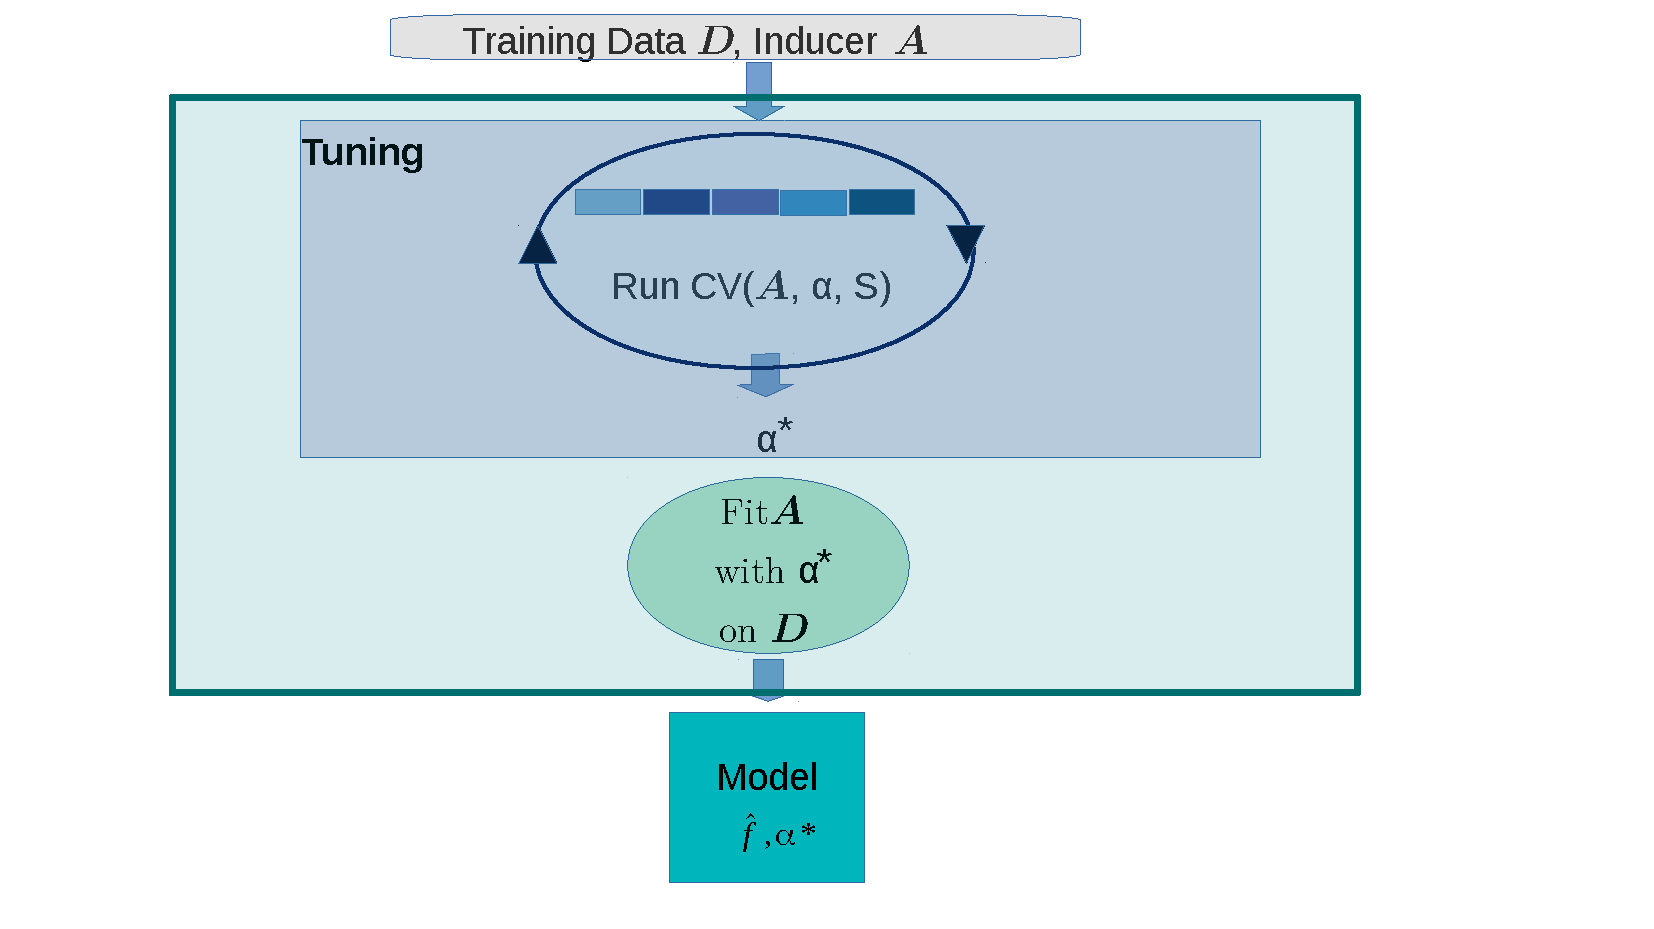
\includegraphics[width=0.8\textwidth]{figure_man/autotune_in_model_fit.pdf}
\end{center}


\framebreak

More precisely: the combined training \& validation set is actually the training test for the \enquote{self-tuning} endowed algorithm. 

\vspace{1cm}
\begin{columns}[c, onlytextwidth]
\column{0.45\textwidth}
\hspace*{-0.3cm}
% FIGURE SOURCE: https://docs.google.com/presentation/d/1kBxfxdUzyUP2-_Y5kWWJ1TnWsm-C4AjHQeTaYPeFo24/edit?usp=sharing
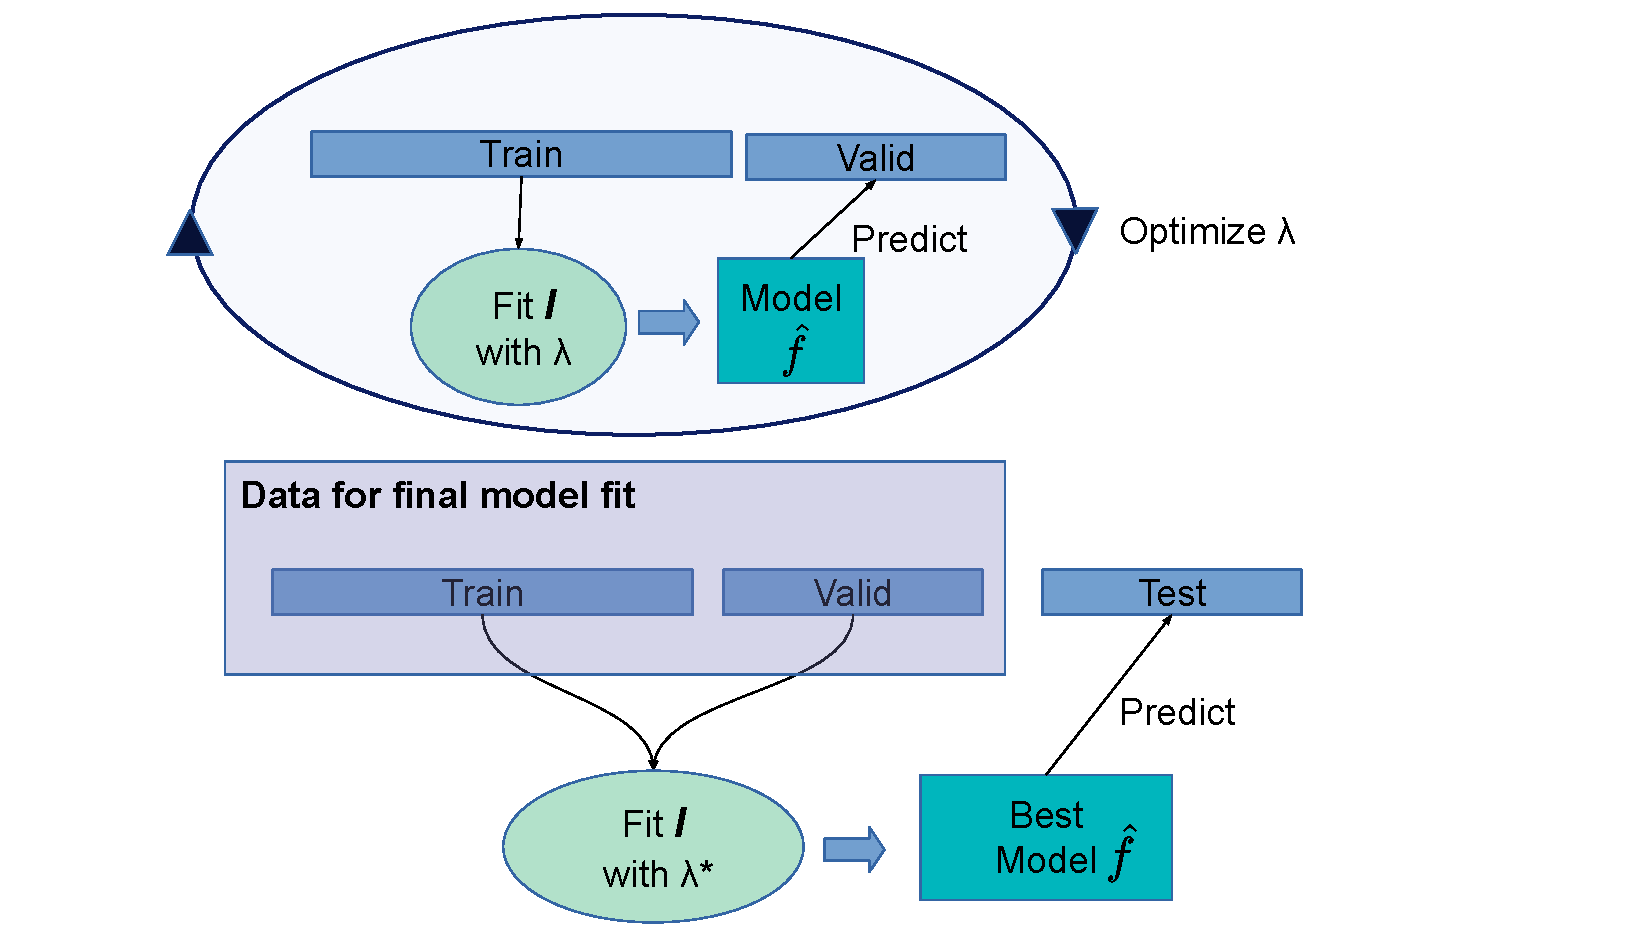
\includegraphics[width=1.5\textwidth]{figure_man/train_valid_test.pdf}
\column{0.45\textwidth}
\hspace*{-0.7cm}
% FIGURE SOURCE: https://docs.google.com/presentation/d/1JUtguuVBgidcqD0IdFFIiKH9zqYzM6YRjCqC53V90dA/edit?usp=sharing
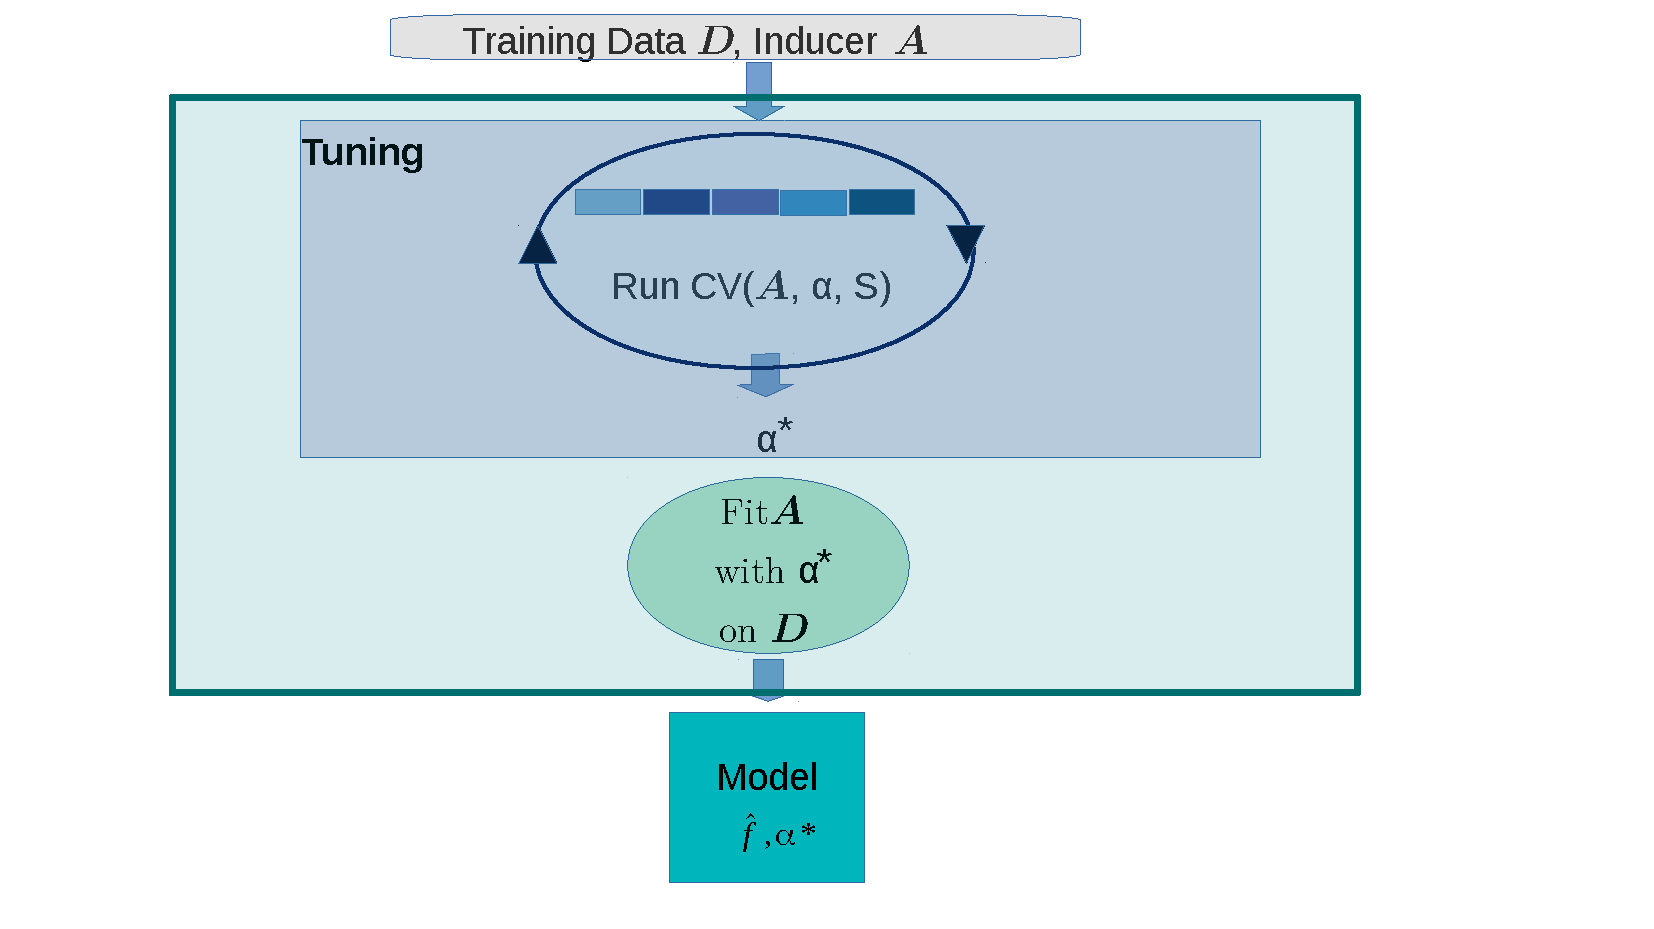
\includegraphics[width=1.5\textwidth]{figure_man/autotune_in_model_fit.pdf}
\end{columns}
\end{vbframe}

\endlecture
\end{document}
